\section{Modelo EA}\label{sec:db}

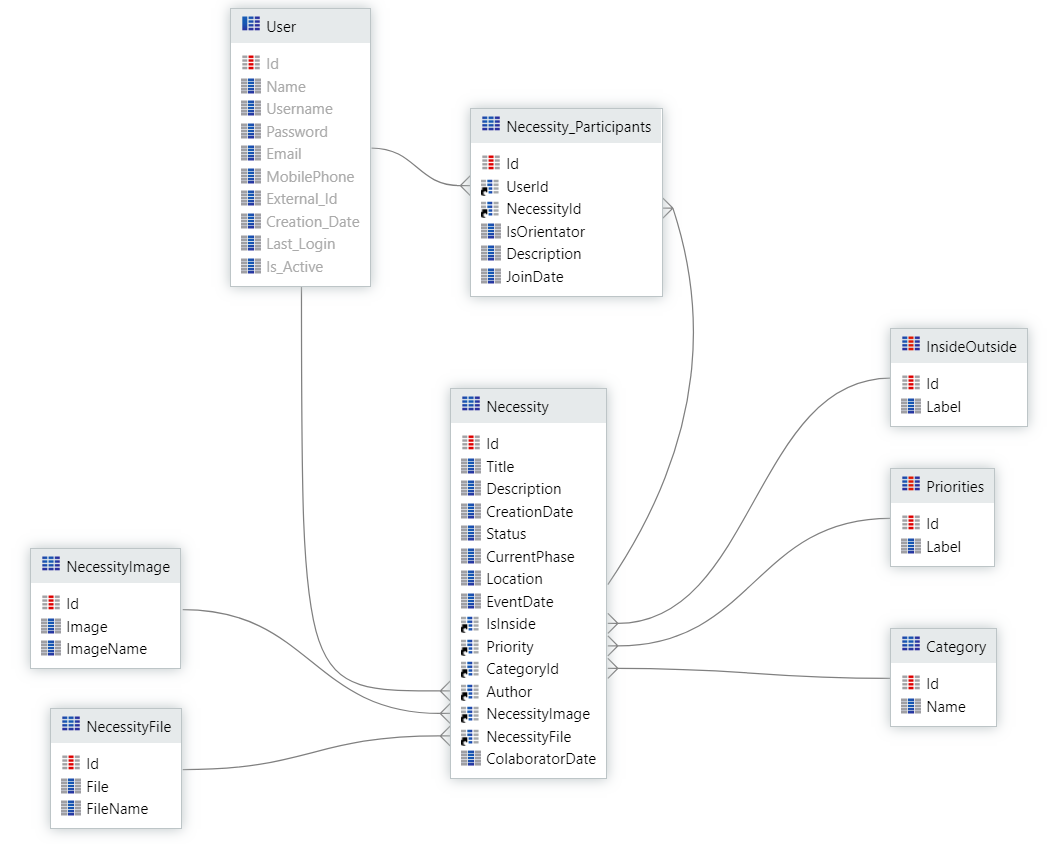
\includegraphics{figures/DataModel}

O conceito predominante no modelo de dados é o de necessidade, representado pela tabela \textit{Necessity}. Uma necessidade é caracterizada por diversos elementos dos quais destacamos o \textit{Status} que corresponde ao estado da mesma, podendo ter por exemplo os valores "Arquivado" ou "A Decorrer", a \textit{CurrentPhase} que indica a fase de candidaturas atual, podendo ser para orientadores ou participantes, e ainda a \textit{ColaboratorDate} que representa a data limite das candidaturas à posição de orientador. 
As tabelas \textit{NecessityImage} e \textit{NecessityFile} existem para o propósito de guardar ficheiros, aliviando a quantidade de dados guardada em cada tuplo \textit{Necessity}, seguindo também as boas práticas da plataforma \textit{OutSystems}. A entidade \textit{InsideOutside} serve para representar a localização das necessidades relativamente a serem  dentro das instalações da empresa ou fora. A mesma, juntamente com a entidade \textit{Priorities} são entidades estáticas cuja funcionalidade é manter dados persistentes na base de dados. Com o objetivo de guardar informação de candidaturas a necessidades, é definida a entidade \textit{Necessity_Participants) que contempla o identificador da mesma, o identificador do utilizador, a descrição associada à candidatura, se esta candidatura é para posição de orientador ou de participante e a data da candidatura. Um utilizador pode ser um participante, um autor ou um orientador da necessidade. Este poderá ainda ter o cargo de administrador, cujos privilégios incluem editar as categorias representadas pela entidade \textit{Category}.